%%%%%%%%%%%%%%%
% TEXTO FEITO %
%   POR LUIZ   %
%   HENRIQUE   %
%%%%%%%%%%%%%%%

\documentclass[a4paper,12pt]{article}

%--- Informações do Documento ---%
\newcommand{\instituicao}{UNESP}
\newcommand{\departamento}{Câmpus de Sorocaba \\ICTS – Instituto de Ciências e Tecnologia}
\newcommand{\curso}{Engenharia de Controle e Automação}
\newcommand{\titulo}{Trabalho 2}
\newcommand{\autor}{Luiz Henrique Corrêa Monteiro, Paulo de Melo Pereira R. Ramalho}
\newcommand{\orientador}{Prof. Dr. Eduardo Godoy Paciência}
\newcommand{\local}{Sorocaba - SP}
\newcommand{\data}{\today}

%--- Pacotes Essenciais ---%
\usepackage[a4paper, left=3cm, right=2cm, top=3cm, bottom=2cm]{geometry}
\usepackage{times}
\usepackage[utf8]{inputenc} % Garante leitura de acentos no código
\usepackage[T1]{fontenc}    % Melhora a fonte final
\usepackage[portuguese]{babel}
\usepackage{hyperref}
\usepackage{titlesec}
\usepackage{lipsum}
\usepackage{fancyhdr} 
\usepackage{graphicx}  
\usepackage{listings}  

%--- CONFIGURAÇÃO DE IMAGENS ---%
\graphicspath{{2-imagens/}} % Agora você não precisa digitar a pasta toda vez

\usepackage{algorithm2e}    
\usepackage{amsfonts, amsthm, amssymb, amsmath, latexsym, bezier, amscd}  
\usepackage{caption}    
\usepackage{subcaption}    
\usepackage{nameref}  
\usepackage{etoolbox}  
\usepackage{float}	
\usepackage{cancel}     
\usepackage{verbatim}			
\usepackage{multirow, array}	
\usepackage{indentfirst}	
\usepackage{xcolor, colortbl}	
\usepackage{pdflscape}    
\usepackage{setspace}  
\usepackage{csquotes} 
\usepackage{multicol} 
\usepackage{enumitem}
\usepackage{romannum}
\usepackage{tcolorbox}

%--- BIBLIOGRAFIA (Ajustado para evitar erro de 'brazil undefined') ---%
\usepackage[backend=biber, style=abnt]{biblatex}
\addbibresource{referencia.bib}

%--- Ajustes de Espaçamento ---%
\titlespacing*{\chapter}{0pt}{-10pt}{20pt}
\titlespacing*{\section}{0pt}{-5pt}{5pt}
\titlespacing*{\subsection}{0pt}{-5pt}{5pt}
\definecolor{backcolour}{rgb}{0.95,0.95,0.92} % Fundo clarinho
\definecolor{codegreen}{rgb}{0,0.6,0}         % Comentários
\definecolor{codegray}{rgb}{0.5,0.5,0.5}      % Números das linhas
\definecolor{codepurple}{rgb}{0.58,0,0.82}    % Strings e Textos
\definecolor{bluekeyword}{rgb}{0.13,0.13,1}   % Palavras-chave padrão
\definecolor{typecolor}{rgb}{0.17,0.57,0.68}  % Tipos customizados (esp_err_t, etc)
\definecolor{macrocolor}{rgb}{0.5,0.0,0.0}    % Macros (ESP_RETURN_ON_FALSE)

% Configuração super "coloridinha" e com quebra de linha
\lstset{
	language=C++,
	backgroundcolor=\color{backcolour},   
	commentstyle=\color{codegreen},
	keywordstyle=\color{bluekeyword}\bfseries,
	numberstyle=\tiny\color{codegray},
	stringstyle=\color{codepurple},
	basicstyle=\ttfamily\scriptsize, % Fonte menor para não sair da folha
	breakatwhitespace=false,         
	breaklines=true,                 % Força a quebra de linhas longas
	captionpos=b,                    
	keepspaces=true,                 
	numbers=left,                    % Números na esquerda
	numbersep=5pt,                  
	showspaces=false,                
	showstringspaces=false,
	showtabs=false,                  
	tabsize=4,
	% Adicionando seus tipos e funções como palavras-chave para colorir!
	morekeywords={uint8_t, size_t, esp_err_t},
	keywordstyle=[2]{\color{typecolor}},
	morekeywords=[2]{ESP_RETURN_ON_FALSE, i2c_master_transmit_receive, i2c_master_transmit, static_cast},
	keywordstyle=[3]{\color{macrocolor}},
	morekeywords=[3]{ESP_RETURN_ON_FALSE}
}
%-------------------------------------------%
\begin{document}
	\pagenumbering{arabic}
	
	%-------------- CAPA -----------------%
	\begin{titlepage}
		\begin{center}
			% Forçamos o caminho completo caso o graphicspath falhe na primeira vez
			
\includegraphics[width=0.8\linewidth]{2-imagens/image.png} 
			
			\vspace*{1cm}
			\textbf{\Large Campus de Sorocaba}\\
			\textbf{\Large ICTS – Instituto de Ciências e Tecnologia}\\[3cm]
			
			\large {Trabalho 1}\\[2cm]
			
			{\large \textbf{Redes de Comunicação Industrial}}\\[4cm]
			\vfill
			\Large\textbf{Discente: \autor}\\
			\textbf{Orientador: \orientador}\\[3.0cm]
			
			\local\\
			2026
		\end{center}
	\end{titlepage}
	
	%--------- FOLHA DE ROSTO ------------%
	\begin{titlepage}
		\begin{center}
			\vspace*{1cm}
			\textbf{\autor}\\[2cm]
			\large \textbf{Programação Remota, Comunicação e Visualização Web usando API Rest HTTP }\\[3cm]
			
			Trabalho apresentado ao Instituto de Ciências e Tecnologia da Unesp, como parte dos requisitos para a conclusão da disciplina em Redes de Comunicação Industrial.\\[2cm]
			
			Orientador: \orientador\\[1cm]
			
			\textit{E-mail} dos alunos autores:\\
			\texttt{lh.monteiro@unesp.br}\\ \texttt{paulo.ramalho@unesp.br}\\[3cm]
			
			\local\\
			2026
		\end{center}
	\end{titlepage}
	
	%--- INPUTS (Sugestão: Renomeie os arquivos para tirar acentos) ---%
	%%Resumo
\section*{Resumo}
%\addcontentsline{toc}{chapter}{Resumo}
Nao preciso fazer o resumo, ent deixo aqui um texto de surpresa para os xeretas de codigo.
	
	\hypersetup{hidelinks}
	\tableofcontents
	\newpage
	
	% Se os arquivos na pasta ainda tiverem acento, use os nomes com acento abaixo. 
	% Se você renomear (recomendado), tire o acento aqui também.
	%%====================================================================%%
%%                         INTRODUÇÃO                                  %%
%%====================================================================%%

\section{Introdução}
\label{sec:introducao}

Atualmente, sistemas de automação e monitoramento utilizam cada vez mais a comunicação em rede para permitir a troca de informações entre dispositivos físicos e aplicações de supervisão. Dentro desse contexto, uma das formas de realizar essa comunicação é através do protocolo HTTP associado a uma API REST, permitindo que diferentes dispositivos realizem operações de envio, consulta e alteração de informações através de uma rede.

Neste trabalho foi desenvolvido um sistema de comunicação entre uma placa ESP32 e uma interface de supervisão construída no Node-RED. O objetivo principal foi realizar a aquisição de variáveis ambientais utilizando um sensor BME280 e disponibilizar essas informações através de uma API REST. Além da aquisição dos sensores, também foi realizada a leitura de um botão físico e o controle remoto de um LED conectado ao ESP32.

O sensor BME280 permite realizar medições de temperatura, umidade relativa e pressão atmosférica. A partir da pressão também é possível realizar uma estimativa da altitude, utilizando como referência um valor conhecido de pressão ao nível do mar. Essas informações são adquiridas pelo ESP32 e posteriormente disponibilizadas para utilização pelo sistema.

A comunicação entre os diferentes elementos foi realizada através de uma rede Wi-Fi utilizando requisições HTTP. A API REST permite realizar a troca de informações entre o dispositivo e o Node-RED, fazendo com que os dados adquiridos pelo ESP32 possam ser apresentados em um dashboard e, no sentido contrário, que comandos realizados através da interface possam alterar o estado do LED.

O Node-RED foi utilizado para construção da interface principal de supervisão. No dashboard desenvolvido é possível acompanhar os valores provenientes do BME280, verificar o estado do botão, visualizar o estado do LED e realizar seu acionamento remotamente. Dessa maneira, foi possível implementar tanto o monitoramento quanto a atuação através da comunicação REST.

Outro requisito desenvolvido durante o trabalho foi a programação remota do ESP32 utilizando OTA (\textit{Over-the-Air}). Após uma primeira programação realizada através da conexão física, o recurso permite enviar novas versões do firmware pela rede Wi-Fi, reduzindo a necessidade de acesso físico ao dispositivo durante atualizações posteriores.

Além dos requisitos principais do trabalho, também foram desenvolvidas algumas funcionalidades extras, que são apresentadas a seguir.
Dessa forma, o desenvolvimento principal do trabalho está concentrado na integração entre ESP32, sensor BME280, API REST e Node-RED, juntamente com a implementação da atualização remota através de OTA. Os demais recursos desenvolvidos são apresentados separadamente como funcionalidades adicionais.



mas distribuídos e conectados.
	%%======%%======%0%======%%=======%%
\vspace{5mm}
\section{Dificuldades e impressões}
%\addcontentsline{toc}{chapter}{Resultados e discussões}

%%======%%======%0%======%%=======%%

%===%===%
%\vspace{1cm}
%===%===%


	%%====================================================================%%
%%                      RECURSOS UTILIZADOS                            %%
%%====================================================================%%
\vspace{5mm}
\section{Recursos utilizados}
\label{sec:recursos}

Para o desenvolvimento do sistema foram utilizados recursos de hardware e software responsáveis pela aquisição das variáveis, comunicação através da rede, visualização das informações e atualização remota do firmware. Entre os principais elementos utilizados estão a placa ESP32, o sensor BME280, o protocolo HTTP, a API REST e a plataforma Node-RED.
\vspace{3mm}
\subsection{Descrição do módulo}

O elemento principal de hardware utilizado no projeto foi uma placa baseada no microcontrolador ESP32. A conectividade Wi-Fi disponível no dispositivo foi utilizada para estabelecer a comunicação com os demais elementos do sistema através da rede.

Além do microcontrolador, o módulo utilizado possui um display OLED, empregado durante o desenvolvimento para apresentar localmente algumas informações relacionadas ao funcionamento do sistema. Dessa forma, foi possível observar diretamente no dispositivo os valores adquiridos e algumas informações relacionadas à conexão.

Para aquisição das variáveis ambientais foi utilizado o sensor Bosch BME280. O sensor permite realizar medições de temperatura, umidade relativa e pressão atmosférica, sendo conectado ao ESP32 através do barramento I$^2$C.

A altitude também é apresentada pelo dispositivo, porém esse valor não corresponde a uma medição direta realizada pelo BME280. Seu valor é estimado através da pressão atmosférica medida e de uma pressão de referência ao nível do mar.

Além do BME280, foi utilizado um botão como entrada digital e um LED como saída. O botão permite enviar para o sistema uma informação proveniente de uma entrada física, enquanto o LED permite verificar o funcionamento da comunicação no sentido contrário, uma vez que seu estado pode ser alterado remotamente.

A Figura \ref{fig:pinout-esp} apresenta o diagrama de pinos utilizado como referência durante a implementação.

\begin{figure}[H]
	\centering
	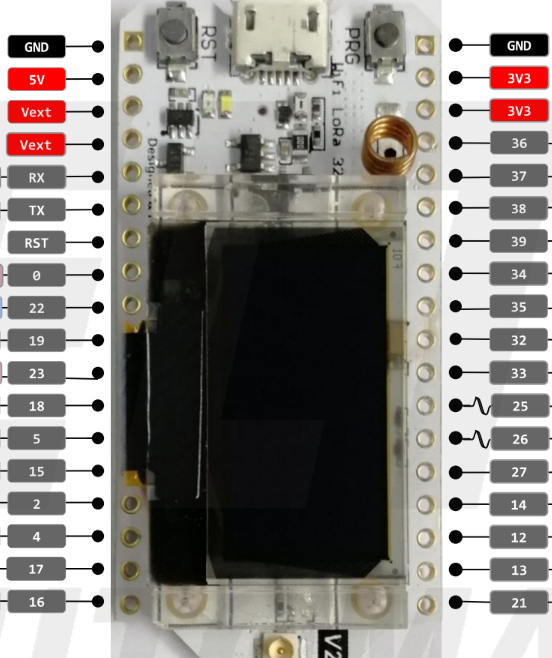
\includegraphics[width=0.3\textwidth, angle=90]{2-imagens/pinout_esp.png}
	\caption{Diagrama de pinos do módulo ESP32 utilizado no projeto.}
	\label{fig:pinout-esp}
\end{figure}


\subsection{Descrição da arquitetura de comunicação}

A arquitetura principal do trabalho foi desenvolvida com o objetivo de permitir a comunicação entre o ESP32 e o Node-RED através de uma API REST utilizando o protocolo HTTP.

O ESP32 é responsável pela aquisição das variáveis físicas. Periodicamente são realizadas leituras do sensor BME280 e do estado do botão. Essas informações são então organizadas pelo firmware e enviadas através da rede.

A API REST é utilizada como meio de comunicação entre os diferentes elementos do sistema. Através de requisições HTTP, os dados adquiridos pelo ESP32 podem ser disponibilizados para o Node-RED, onde são posteriormente tratados e apresentados ao usuário.

De maneira simplificada, o fluxo relacionado à aquisição das informações pode ser representado por:

\begin{center}
	\textbf{BME280 / Botão $\rightarrow$ ESP32 $\rightarrow$ API REST $\rightarrow$ Node-RED}
\end{center}

Além da aquisição, foi implementada uma comunicação no sentido contrário para permitir a atuação remota sobre o LED. Nesse caso, o usuário realiza uma alteração através do dashboard do Node-RED e o comando correspondente é disponibilizado através da API para o ESP32.

O fluxo de atuação pode ser representado por:

\begin{center}
	\textbf{Node-RED $\rightarrow$ API REST $\rightarrow$ ESP32 $\rightarrow$ LED}
\end{center}

Essa estrutura permite demonstrar duas situações diferentes de comunicação. Na primeira, o ESP32 atua como origem das informações adquiridas pelos sensores. Na segunda, o dispositivo recebe uma informação proveniente da interface e realiza uma ação física.

A utilização de uma API REST permite separar a aquisição realizada pelo dispositivo da apresentação realizada no Node-RED. Dessa maneira, a comunicação ocorre através de rotas e mensagens definidas, sem a necessidade de uma ligação direta entre os elementos da interface e cada função implementada no firmware.

\begin{figure}[H]
	\centering
	\resizebox{\linewidth}{!}{%
		\begin{tikzpicture}[
			node distance=1.1cm,
			>=Latex,
			bloco/.style={
				rectangle,
				draw=black,
				rounded corners=3pt,
				minimum width=2.6cm,
				minimum height=1.2cm,
				align=center,
				font=\small
			},
			seta/.style={
				->,
				thick
			}
			]
			
			% --------------------------------------------------------
			% Blocos principais
			% --------------------------------------------------------
			
			\node[bloco] (sensores) {
				\textbf{Aquisição}\\
				BME280 / Botão
			};
			
			\node[bloco, right=of sensores] (esp32) {
				\textbf{ESP32}\\
				Firmware
			};
			
			\node[bloco, right=of esp32] (api) {
				\textbf{API REST}\\
				HTTP
			};
			
			\node[bloco, right=of api] (nodered) {
				\textbf{Node-RED}\\
				Dashboard
			};
			
			
			% --------------------------------------------------------
			% Fluxo de aquisição
			% --------------------------------------------------------
			
			\draw[seta]
			(sensores) --
			node[above, font=\scriptsize] {Leitura}
			(esp32);
			
			\draw[seta]
			(esp32) --
			node[above, font=\scriptsize] {Dados}
			(api);
			
			\draw[seta]
			(api) --
			node[above, font=\scriptsize] {HTTP}
			(nodered);
			
			
			% --------------------------------------------------------
			% LED
			% --------------------------------------------------------
			
			\node[bloco, below=2.2cm of esp32] (led) {
				\textbf{Atuador}\\
				LED
			};
			
			
			% --------------------------------------------------------
			% Fluxo de atuação
			% --------------------------------------------------------
			
			\draw[seta]
			(nodered.south) -- ++(0,-0.8)
			-|
			node[pos=0.25, below, font=\scriptsize] {Comando}
			(api.south);
			
			\draw[seta]
			(api.south) -- ++(0,-1.6)
			-|
			node[pos=0.25, below, font=\scriptsize] {Estado do LED}
			(esp32.south);
			
			\draw[seta]
			(esp32) --
			node[right, font=\scriptsize] {Acionamento}
			(led);
			
			
			% --------------------------------------------------------
			% Identificação dos fluxos
			% --------------------------------------------------------
			
			\node[
			above=0.55cm of api,
			font=\small\bfseries
			] {Fluxo de aquisição};
			
			\node[
			below=2.1cm of api,
			font=\small\bfseries
			] {Fluxo de atuação};
			
		\end{tikzpicture}%
	}
	\caption{Arquitetura principal de comunicação entre o ESP32, a API REST e o Node-RED.}
	\label{fig:arquitetura_principal}
\end{figure}

\subsection{Metodologia de implementação}

A implementação foi realizada inicialmente através do desenvolvimento da comunicação necessária entre o ESP32 e a API REST. O firmware foi preparado para realizar a leitura do sensor BME280 e do botão, além de permitir o acionamento do LED.

Após a leitura correta das variáveis, foi realizada a implementação das requisições HTTP necessárias para a troca de informações. Nessa etapa foram realizados testes para verificar o envio da telemetria e a consulta do estado do atuador.

Em seguida foi desenvolvido o fluxo no Node-RED. A interface passou a consultar as informações disponibilizadas pela API e apresentar os valores de temperatura, umidade e pressão, além dos estados correspondentes ao botão e ao LED.

Posteriormente foi implementado o caminho contrário da comunicação, permitindo que o estado do LED fosse alterado através do dashboard. Dessa forma, foi possível verificar a comunicação tanto no sentido ESP32 para Node-RED quanto no sentido Nodered para ESP32.

Por último, foi configurada a atualização remota do firmware utilizando OTA. Após a programação inicial através da conexão física, foram realizados testes de atualização utilizando a rede Wi-Fi.

Após o funcionamento dos requisitos principais, foram desenvolvidas separadamente algumas funcionalidades adicionais, apresentadas posteriormente na subseção de desenvolvimento extra.



	
%%======%%======%0%======%%=======%%
\vspace{5mm}
\section{Programação}
%\addcontentsline{toc}{chapter}{Materiais e métodos}

%%======%%======%0%======%%=======%%
Todo o código desenvolvido e utilizado, está presente no repositório do Git-Hub, e pode ser acessado clicando \href{https://github.com/rick-12q/Trabalho_02_RIC}{AQUI}.
\vspace{5mm}
\subsection{Programação do ESP32}

\vspace{5mm}
\subsection{Construção da interface Node-Red}

\vspace{5mm}
\subsection{Realização do OTA}


\vspace{5mm}
\subsection{Desenvolvimento extra}


	%%======%%======%0%======%%=======%%

\section{Conclusão}
%\addcontentsline{toc}{chapter}{Conclusão}

%%======%%======%0%======%%=======%%


	
	%------------ REFERÊNCIAS ---------------%
	\nocite{*}
	\printbibliography 
	
	%------------ APÊNDICES -----------------%
	%%%======%%======%0%======%%=======%%

\section{Apêndices}
%\addcontentsline{toc}{chapter}{Apêndices}

%%======%%======%0%======%%=======%%

%===%===%
%\vspace{1cm}
%===%===%

	
\end{document}